\section{Parallel FEA Simulations Using GPU }\label{work-overview}

\subsection{General purpose computation with GPU's}

  General-purpose computing on graphics processing units (GPGPU) is the technology that allows utilization of the Graphical Processing Units (GPU's) non-graphical computational tasks. Traditionally, GPU's are only used for rasterization and per-vertex transformation in graphical applications. However, the high-throughput hardware comprising the GPU's is useful not only for rendering purposes. Assuming that the computations can can be subdivided into considerably small chunks the processing can be parallelized using the many-core GPU architecture.

  An algorithm is run in parallel on a set of object. In the context of GPGPU such algorithm is named a \textit{kernel}. Each of the instances of the kernel is being run in a single \textit{thread}.

  Finite elements is an example of a task that requires large amounts of processing. In the case of a real-time interactive simulation, the quality of the resulting simulations may depend on the maximum rate at which a simulation can be performed. Therefore, considering that explicit FEM schemes and especially TLED is remarkably parallelizable GPGPU implementation presents great potential on accelerating the simulation rates.

  The power GPGPU can be accessed through a number of available API's. This section is aimed at discussing the available options and justifying the final choice of API for parallel implementation of the TLED scheme. The details of the implementation are provided further.

\subsection{C++ AMP, OpenCL and CUDA}

  \subsubsection{C++ AMP}

  C++ AMP is an abstraction layer over CUDA, OpenCL and traditional operating system threading API's. It allows simplifying the computation set-up procedures. It can be used to parallelize code regardless of the underlying architecture or hardware, which means that both multi-core CPU's and many-core GPU's are accessible.

  Another important aspect of C++ AMP is that the parallel kernels are written within platform C++ code with minimal changes to the language. This is another advantage for the choice of this framework as the parallelization library for the TLED GPU implementation.

  \paragraph{Discussion} It has been reported \cite{Wong-perf:2010} that the abstraction layer carries a performance overhead. Also, we were unable to find any existing C++ AMP finite element implementations. This may indicate that the abstraction layer actually complicates FEM implementation, as the developer requires low-level access to the hardware.

  \subsubsection{CUDA}

  CUDA is a proprietary NVidia \cite{nvidia-cuda} GPGPU parallelization API. It is very popular in many areas including scientific research. This is due the fact that it provides a usable interface. Like C++ AMP it also provides a much simpler integration with host machine code. The parallel kernels can be written inside C++ code using the \textit{\_\_global\_\_} keyword. This makes developing parallel applications much simpler.

  \paragraph{Discussion}
  % The API finds considerable use in scientific research \cite{Joldes2010, Taylor2008, Johnsen2014}.
  High accuracy and performance make the it appealing as the target parallelization library. However, the proprietary nature of CUDA makes it less attractive as it implies non-optional requirement of using an NVidia GPU. Also, worth mentioning that only GPU parallelization is supported. Another important fact is that CUDA has already been used to implement TLED as presented in \cite{Johnsen2014}. We believe that an alternative implementation may present more scientific merit.

  \subsubsection{OpenCL}

  OpenCL is an open-source cross-platform parallel processing API supervised by Khorons Group \cite{khronos-opencl}. The API is similar to OpenGL and provides low-level access to the hardware. It is different from the other API's discussed above. It does not allow embedding kernel code inside. This, however, can be fixed by using third-party tools \cite{Lawlor2003} that extract and compile OpenCL kernels from the host code. It is however similar to C++ AMP in terms of following a heterogeneous parallel computation model \cite{Stone2010}.

  \paragraph{Discussion} Due to the fact that it is a lower-level heterogenous API, OpenCL has certain drawbacks. The fact that the parallel kernels need run on the wide range of supported hardware, implies that all OpenCL code needs to be loaded dynamically and precompiled on application start-up. However, this is a minor complication, compared to its advantages. The favor is given to OpenCL to its cross-platformity and high-performance. Additionally, there are yet to be created any parallel implementations of TLED scheme using OpenCL.

\subsection{TLED using OpenCL}

  The implementation by \cite{Johnsen2014} uses CUDA to parallelize their FE simulation routines and offload them to the GPU. It has been decided that OpenCL presents a more appealing alternative for the API of choice.

  \subsubsection{Adapting the TLED algorithm}\label{gpu-adapting-tled}

  \paragraph{Splitting work}

  The algorithm presented in section \ref{fea-algorithm} does not account for a parallel implementation. The whole of the algorithm cannot be run in parallel in a single OpenCL kernel. As seen on Figure \ref{gpu-kernels} The internal force calculation needs to be in a separate kernel and be completed before the \textit{deformation update} kernel can be run. The important difference and ultimately the reason for the separation is in the fact that the two kernels are run on different objects. The internal forces are calculated per element and thus the kernel is run in $n$ threads, where $n$ is the number of elements in the finite element mesh. The deformation update kernel however uses the accumulated force to integrate over time and update the deformation of every node. The latter kernel is run $n$ times, where $n$ is the number of nodes in the finite element mesh.

  \begin{figure}
    \centering
      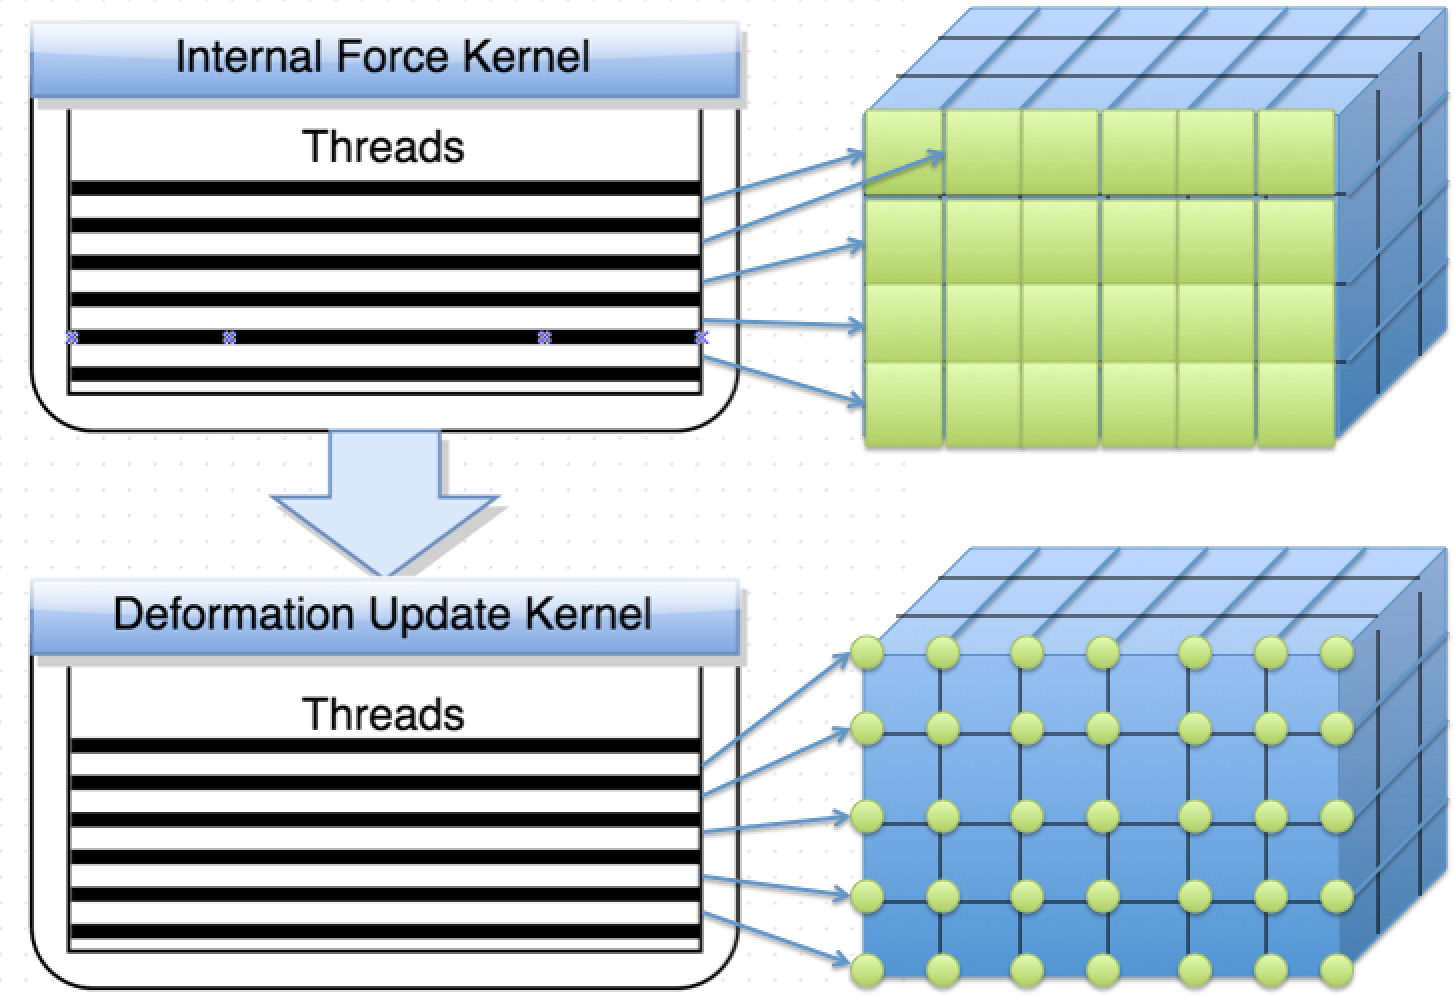
\includegraphics[width=90mm]{sections/methodology/images/gpu/kernels.png}
    \caption{\label{gpu-kernels} GPU based implementation algorithm flow. Element-wise internal force calculation needs to be run in a separate thread, before performing per-node deformation update.}
  \end{figure}

  \paragraph{Pure C kernels}

  The chosen OpenCL API is most suitable in parallelizing pure C kernels. The CPU version of our TLED implementation is C++ based. This required converting the internal force calculation part of our algorithm into a pure C version. This version was then included into an OpenCL kernel.

  \paragraph{Flat data-structures}

  It is considered best-practice to avoid using standard data-structures used in CPU programs when performing GPGPU computations \cite{opencl_programming_munshi}. Therefore, all data-structures have been redesigned to incorporate buffered data, also known as \textit{structs of arrays} paradigm. The implementation of the principle in our system is illustrated on Figure \ref{gpu-structs-vs-arrays}. The class representing a finite element does not contain the data, but only points to the location in the buffer containing all the data of a particular class field.

  \begin{figure}
    \centering
      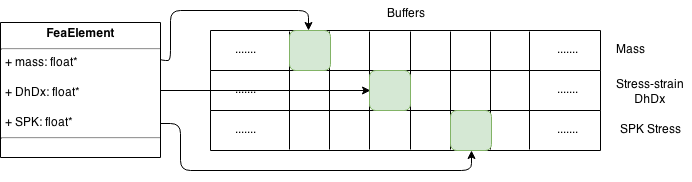
\includegraphics[width=120mm]{sections/methodology/images/gpu/structs-vs-arrays.png}
    \caption{\label{gpu-structs-vs-arrays} Modified data-structure layout for the GPU based implementation following \textit{structs of arrays} principle.}
  \end{figure}


  \subsubsection{Efficient memory utilization}

  The GPU implementation of the TLED force calculation in the OpenCL kernel is not memory bound but computation bound. However, it is important to minimize the memory access overhead, as otherwise performance may suffer considerably.

  All modern processing units have a memory hierarchy. Typically the lowest level of memory hierarchy is the global omni-accessible shared memory. The highest in the hierarchy is the private memory accessibly only to the core that it belongs to. OpenCL API provides a specific way of using the GPU memory hierarchy \cite{opencl_programming_munshi} as seen in Figure \ref{gpu_opencl_memory_hierarchy}. The private memory provides small by very fast memory. The global memory is accessible from all threads, but carries large access time overhead.

  \begin{figure}
    \centering
      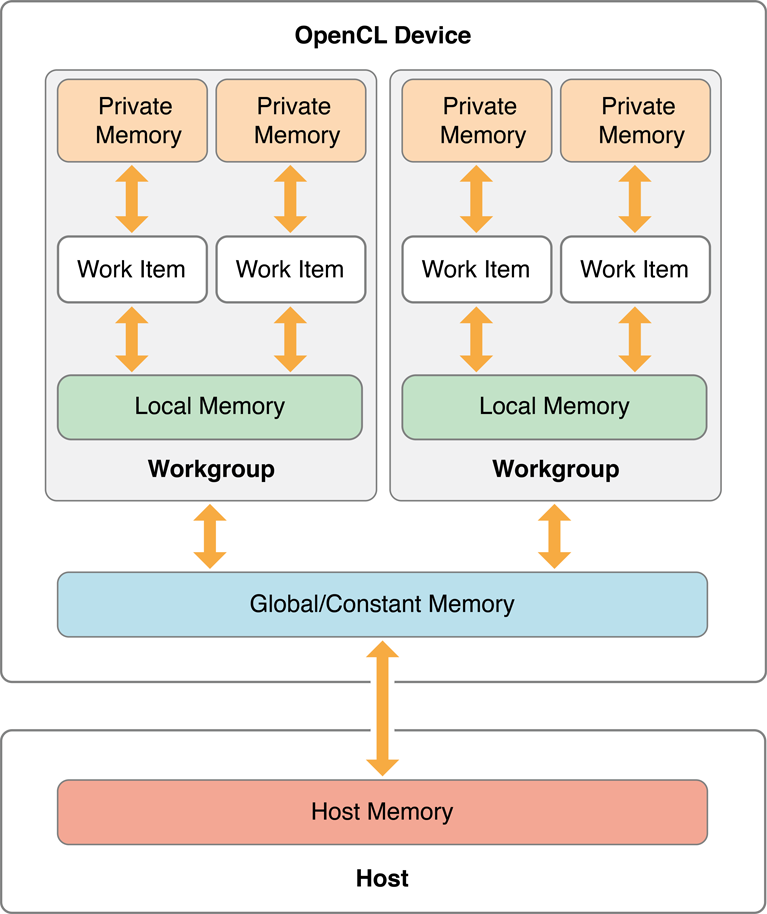
\includegraphics[width=90mm]{sections/methodology/images/gpu/opencl_memory_hierarchy.png}
    \caption{\label{gpu_opencl_memory_hierarchy} OpenCL memory model. The private memory provides small by very fast memory. The global memory is accessible from all threads, but carries large access time overhead.}
  \end{figure}

  Our implementation utilizes this hierarchy by avoiding constant requests to the global memory. The \textit{internal forces} kernel has several buffer inputs in global memory. Certain chunks of the buffers are accessed repeatedly in the kernel. To avoid memory access overhead we copy the whole chunk into the private memory of the thread for further access in the thread.

  \subsubsection{Data-race conditions}

  Any parallelized algorithm that requires writing to a global location in memory suffers from data-race problem. The issue occurs in the case of two or more threads accessing the same location in memory, when at least one of them is modifying the said memory stored at the location. The non-deterministic result of the operation is also known as \textit{undefined behavior}. It should be noted that reading from a common location does not carry any of the overhead.

  Figure \ref{gpu-data-race} illustrates the problem. The threads representing parallel processes perform read and write operations. However, the operations are performed on different occasions and no issues arise. However, in the unpredictable even when two threads modify the same memory location based on the current value (consider C++'s $+=$ operator) the result of the operation in both cases depends on which of the threads was first. The access order information is deliberately inaccessible.

  \begin{figure}
    \centering
      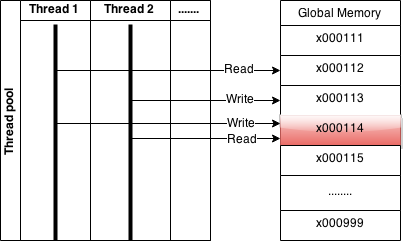
\includegraphics[width=100mm]{sections/methodology/images/gpu/data-race.png}
    \caption{\label{gpu-data-race} Data-race condition in a parallel application when two or more threads are attempting to access a memory location with one of the threads making a modification to memory.}
  \end{figure}

  In the particular case of the the OpenCL TLED kernel the only place when the data-race condition occurs is when the calculated forces are stored for each node. Note, that this problem arises from the fact that some of the elements share nodes. This means that when two or more element threads will try to modify the force value for a particular node.

  In order to overcome this issue use a similar approach to the one used in \cite{Johnsen2014}. The approach is to replicate the nodal force information for each element. This means that the amount of data required is proportional to the number of nodes in the type of finite element used to represent simulated mesh.

  We adopt a simpler memory layout for replicated nodal forces buffer as compared to the one used in \cite{Johnsen2014}. The paper states that they use a lookup table to find the addresses of the nodal forces. The memory layout adopted in BirthView is continuous and the nodes of a single element are adjacent in memory. Lets consider the instance of a hexahedral mesh, where each element consists of a eight nodes. This results in an eight fold increase in the amount of memory required to store the nodal force values. Fortunately, the modern hardware is capable of storing considerable amount of data. As seen in Figure \ref{gpu-data-race-solution} each element corresponds to a set of eight nodal forces.

  \begin{figure}
    \centering
      \includegraphics[width=100mm]{sections/methodology/images/gpu/data-race-solution.png}
    \caption{\label{gpu-data-race-solution} The memory layout of the nodal forces buffer.}
  \end{figure}
